\univlogo

{\Huge March 30}\vspace{5mm}

\section*{Phase Lock Loop}

The droop control reminds me of a technology named Phase Lock Loop (PLL), which is used to synchronize phases of two waves.

It consists of three parts: \textbf{Phase Detector}, \textbf{Low-Pass Filter} and \textbf{Voltage Controlled Oscillator}.

\begin{figure}[H]
\centering
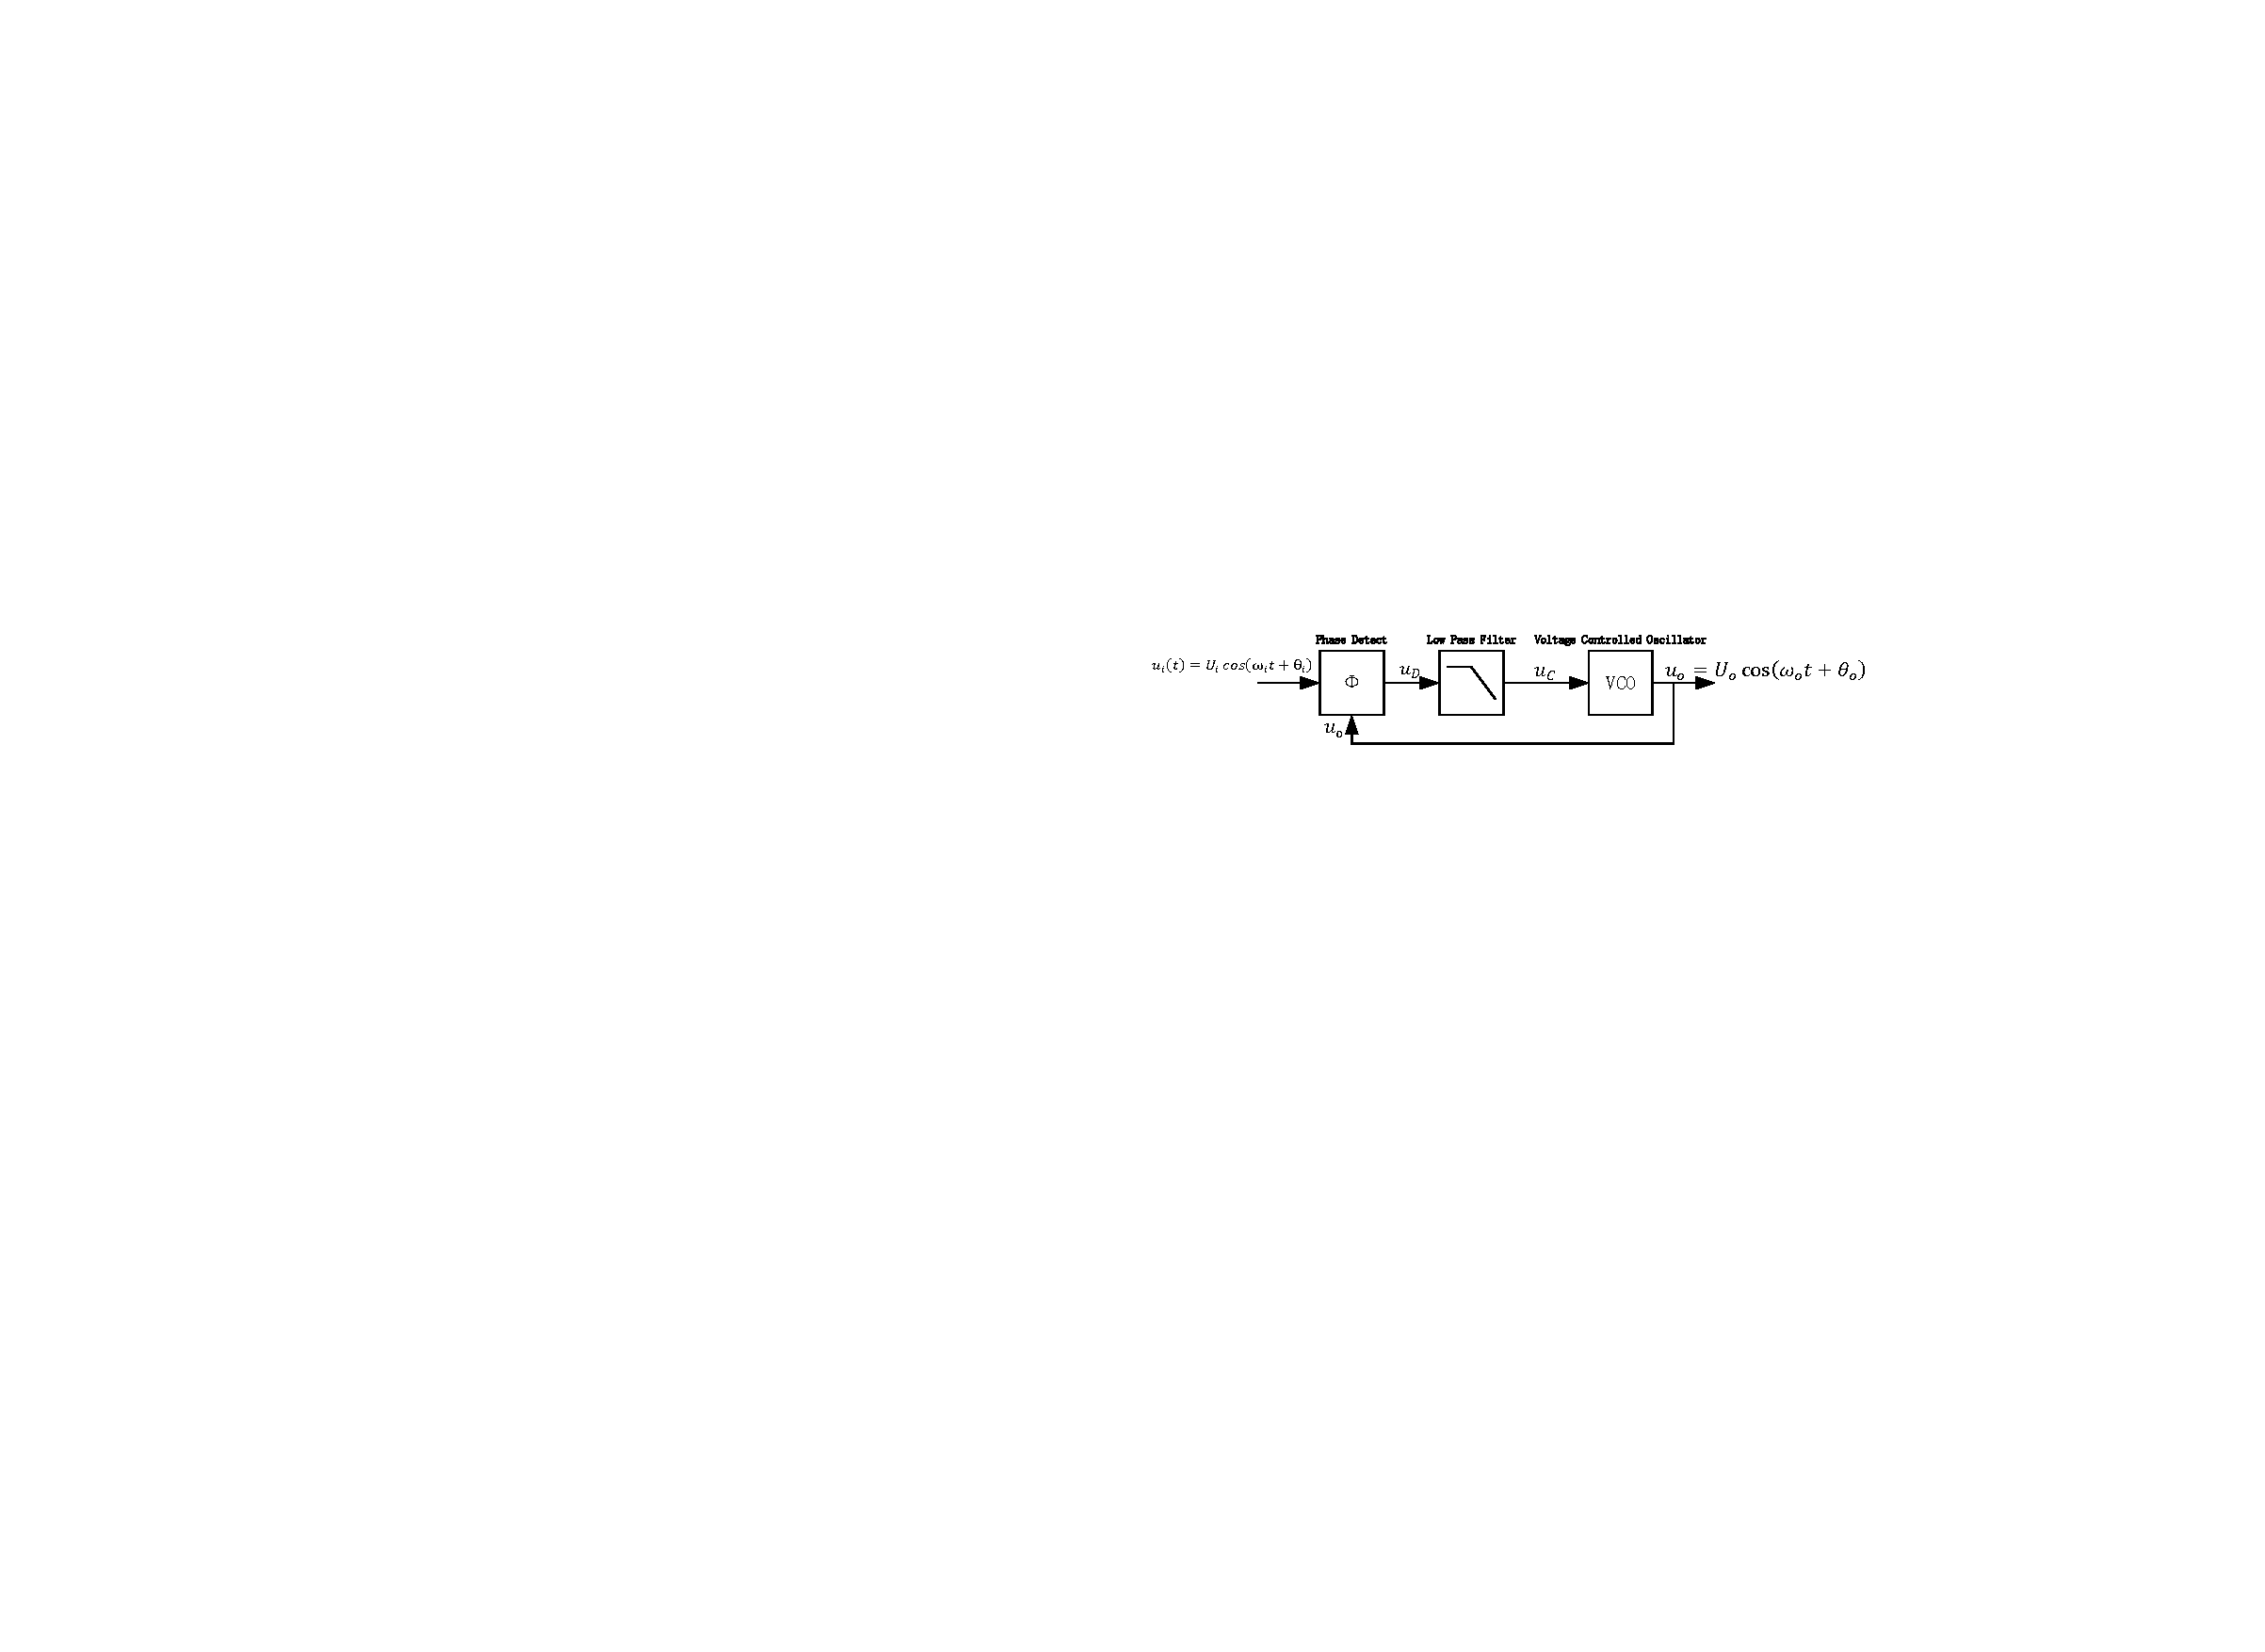
\includegraphics[width=1\textwidth]{./2023Mar/PLL.pdf}
\caption{PLL}
\label{PLL}
\end{figure}

\subsection*{Phase Detector}

To obtain the phase difference information, the PD multiplies the two input waveforms.

\begin{equation}
\begin{aligned}
    u_D&=K_Du_i(t)\cdot u_o(t) \\
    &=K_DU_iU_o\cos{(\omega_i t+\theta_i(t))}\cos{(\omega_o t +\theta_o(t))}\\
    &=\cfrac{K_DU_iU_o}{2}[\cos{((\omega_i+\omega_o)t+(\theta_i(t)+\theta_o(t)))}+\cos{((\omega_i-\omega_o)t+(\theta_i(t)-\theta_o(t))}]
\end{aligned}
\end{equation}

\subsection*{Low-Pass Filter}

The sum frequency component of the above equation is filtered out with a LPF, and the remaining differential frequency component is used as the input control voltage of the VOC.

\begin{equation}
\begin{aligned}
    u_C=U_{dm}\cos{((\omega_i-\omega_o)t+(\theta_i(t)-\theta_o(t)))}
\end{aligned}
\end{equation}

The \textbf{instantaneous phase difference} $\theta_d$ is:

\begin{equation}
\begin{aligned}
    \theta_d=(\omega_i-\omega_o)t+\theta_i(t)-\theta_o(t)
\end{aligned}
\end{equation}

By the way, the \textbf{instantaneous frequency difference} is:

\begin{equation}
\begin{aligned}
    \cfrac{\mathrm{d} \theta_d}{\mathrm{d} t}=\omega_i-\omega_o+\cfrac{\mathrm{d} [\theta_i(t)-\theta_o(t)]}{\mathrm{d} t}
\end{aligned}
\end{equation}

When $\cfrac{\mathrm{d} \theta_d}{\mathrm{d} t}=0$, it means that the phase-locked loop enters a phase-locked state, at which the frequency and phase of the output and input signals remain in a constant state, and $u_C(t)$ is a constant value. When the above equation is not equal to zero, it means that the phase of the phase-locked loop is not yet locked, the frequency of the input and output signals are not equal, and $u_C(t)$ changes with time.

The voltage-controlled characteristic of a VCO states that its oscillation frequency $\omega_u$ is centered on $\omega_0$ and varies with the input signal voltage $u_C(t)$. 

\begin{figure}[H]
\centering
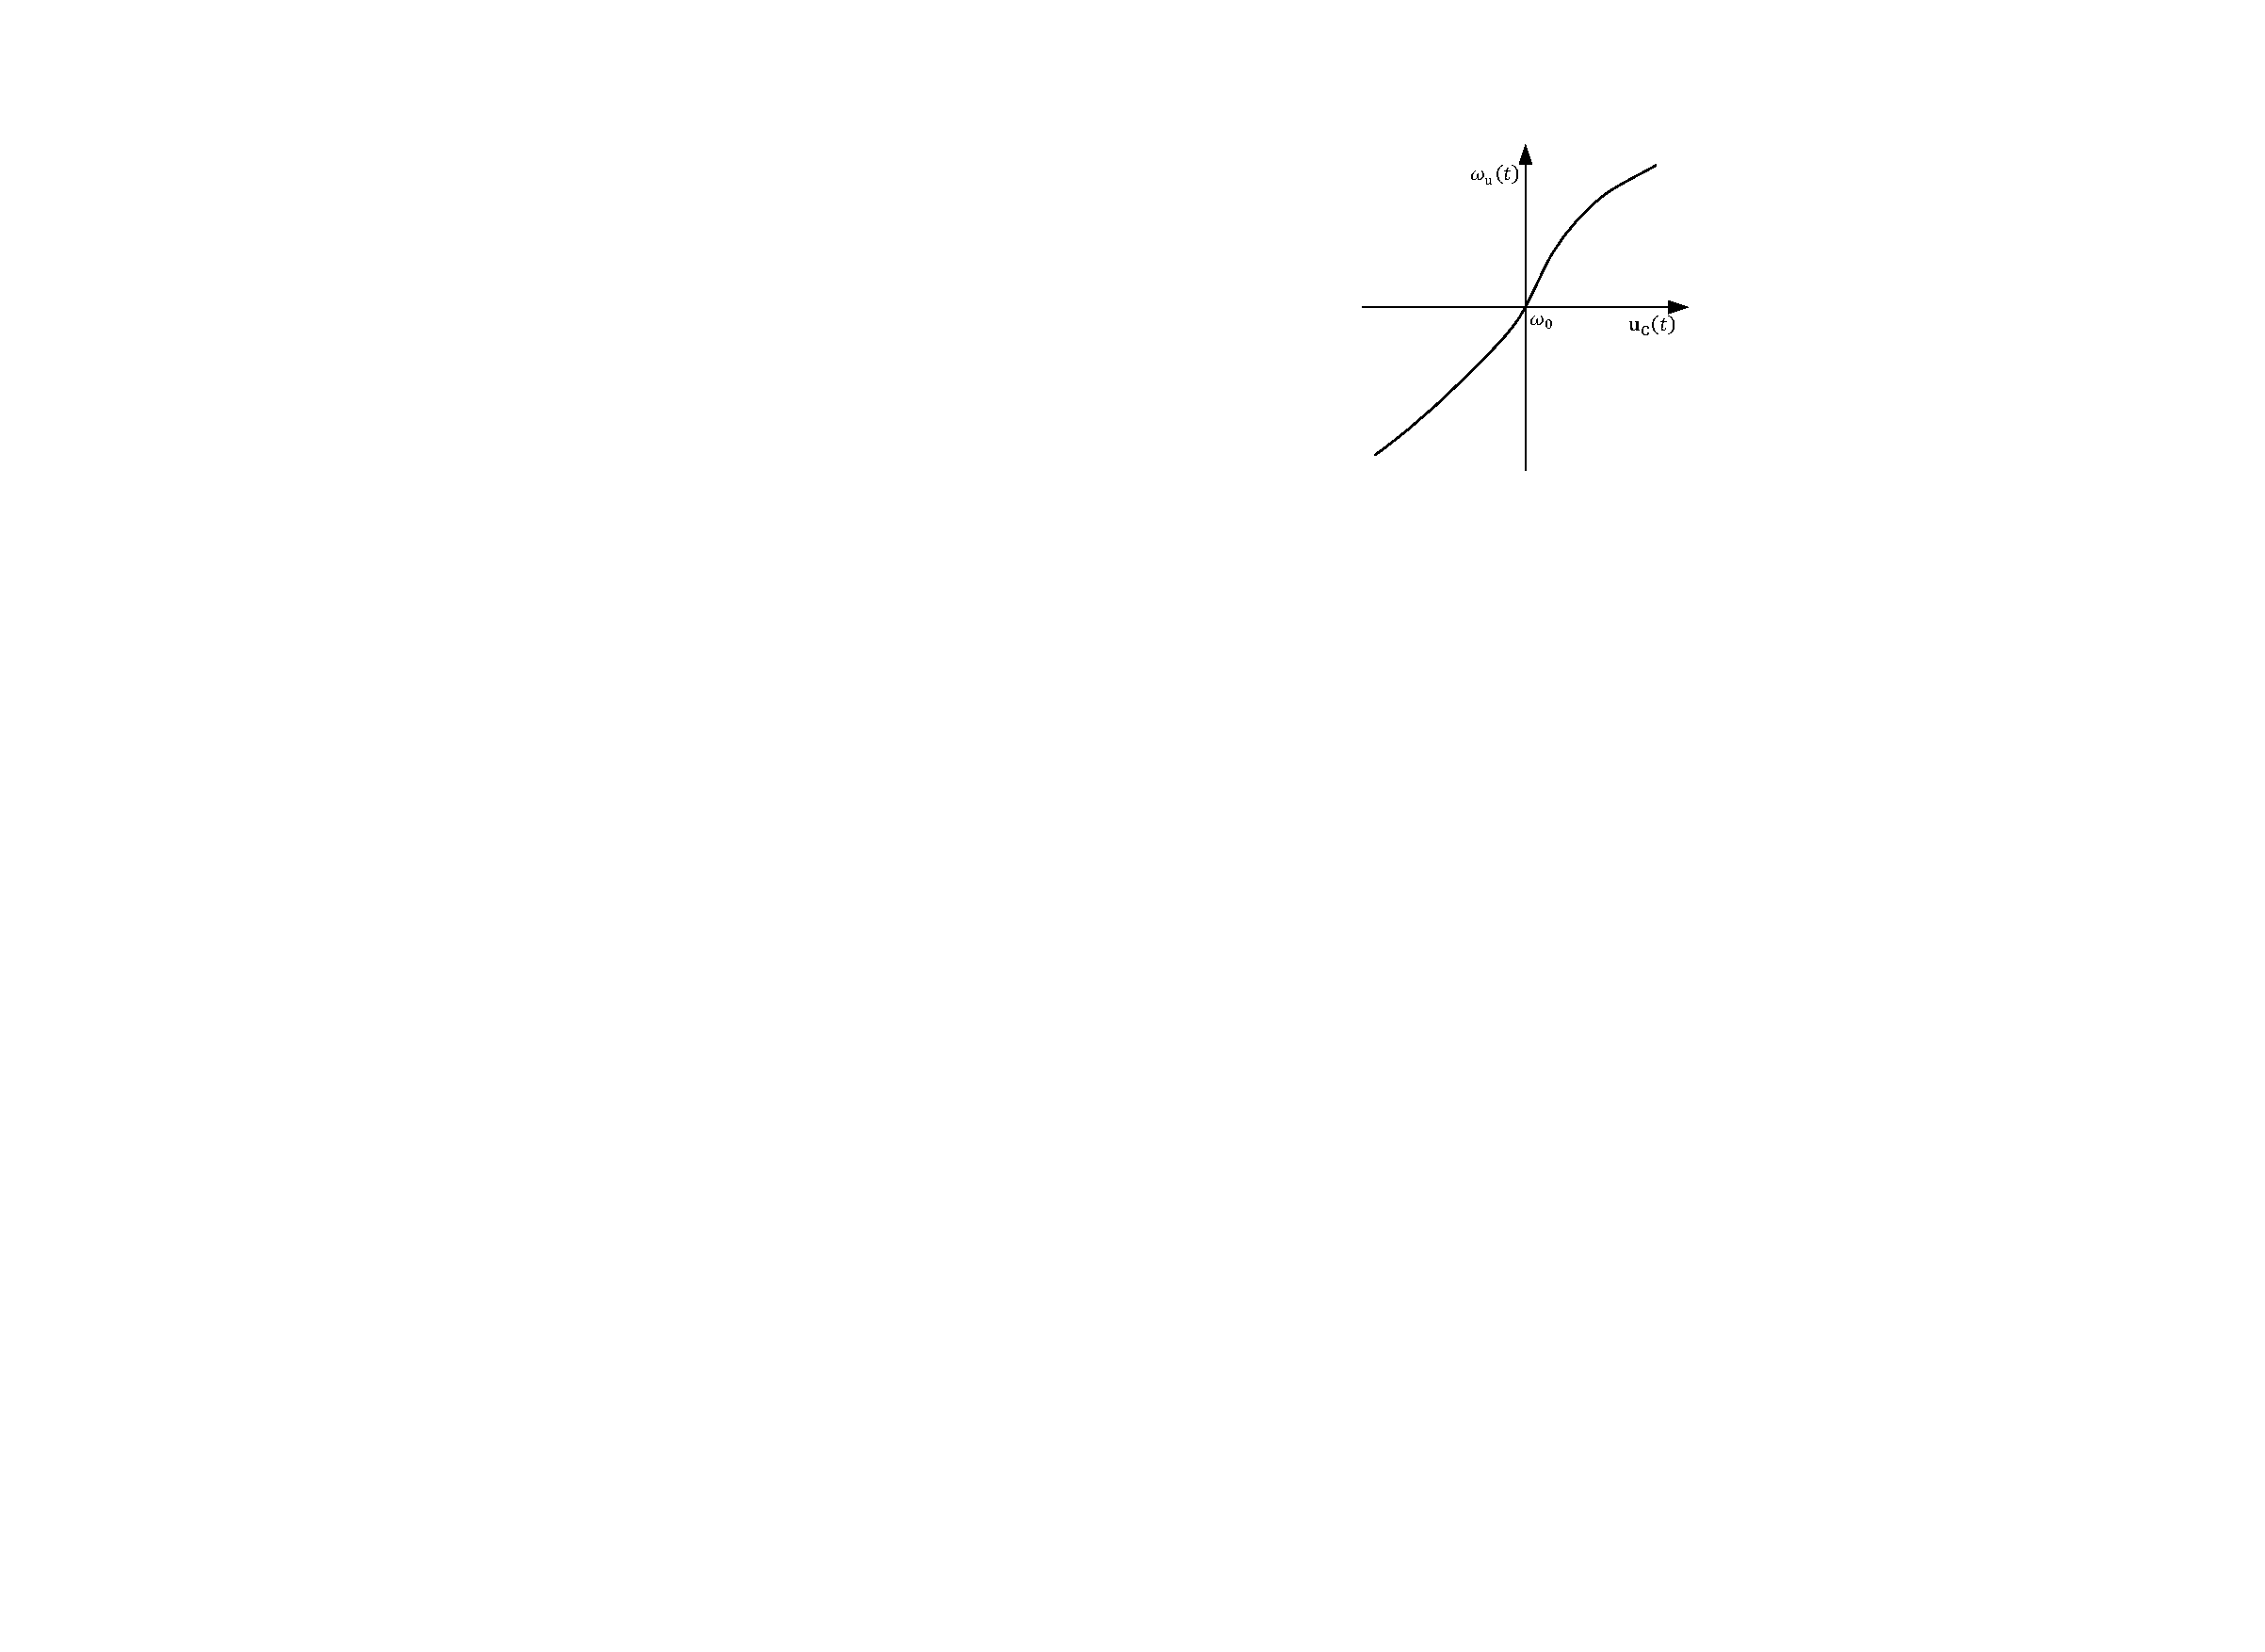
\includegraphics[width=0.4\textwidth]{./2023Mar/VCO.pdf}
\caption{VCO}
\label{VCO}
\end{figure}

The expression of this characteristic is given by:

\begin{equation}
\begin{aligned}
    \omega_u(t)=\omega_0+K_0u_C(t)
\end{aligned}
\end{equation}
    
The above equation shows that when $u_C(t)$ varies with time, the oscillation frequency $\omega_u$ of the voltage controlled oscillator also varies with time, and the phase-locked loop enters into "frequency traction", automatically tracking the frequency of the captured input signal, so that the phase-locked loop enters the locked state and keeps the state of $\omega_o=\omega_i$ unchanged.

